%********************************************************************************
\documentclass{article}
\usepackage{etex}
\reserveinserts{28}

%-------------------------------------------------------------------------------
%--- PACKAGES
%-------------------------------------------------------------------------------
\usepackage{url}
\usepackage{longtable}
\usepackage{booktabs}
\usepackage{bold-extra}
\usepackage{rotating}
\usepackage{dcolumn}
%\usepackage{chronology}
\usepackage{color}
\pagecolor{white}
\usepackage{pdfpages}
\usepackage{lastpage}
\usepackage{lscape}
\usepackage{lineno}
\usepackage{setspace}
\usepackage{amsmath}
\usepackage{amssymb}
\usepackage{breqn}
\usepackage{appendix}
\usepackage{natbib}
\usepackage[capposition=top]{floatrow}
\usepackage{graphicx}
\usepackage{epsfig}
\usepackage{epstopdf}
\usepackage{multirow}
\usepackage{titletoc}
\usepackage{wrapfig}
\usepackage{blindtext}
\usepackage{subcaption}
\usepackage{subfloat}
\usepackage{xr}
\externaldocument{MMREducation_BhalotraClarke}


%-------------------------------------------------------------------------------
%--- SPECIFICATIONS (MARGINS, TOC, BIBLIO)
%-------------------------------------------------------------------------------
\setlength\topmargin{-0.375in}
\setlength\textheight{8.8in}
\setlength\textwidth{5.8in}
\setlength\oddsidemargin{0.4in}
\setlength\evensidemargin{-0.5in}

\bibliographystyle{abbrvnat}
\bibpunct{(}{)}{;}{a}{,}{,}
\newcommand{\MMRfolder}{"."}


\titlecontents{section}
[0pt]
{}%
{\contentsmargin{0pt}
    \thecontentslabel\enspace%
    }
{\contentsmargin{0pt}}
{\titlerule*[.5pc]{.}\contentspage}
[]

\renewcommand\figurename{Appendix Figure}
\renewcommand\tablename{Appendix Table}
\renewcommand\thesection{\Alph{section}}
\renewcommand*{\thepage}{A\arabic{page}}
\renewcommand*{\theequation}{A\arabic{equation}}


%-------------------------------------------------------------------------------
%--- FRONT PAGE
%-------------------------------------------------------------------------------
\begin{document}
\begin{spacing}{1.4}

\begin{center}
\textbf{ONLINE APPENDICES} \\
\vspace{4mm}
From the paper: \\
\vspace{6mm}
       {\large \textsc{Maternal Education and Maternal Mortality:
       Evidence from a Large Panel and Various Natural Experiments}} \\
Sonia Bhalotra and Damian Clarke
\end{center}

\tableofcontents


%-------------------------------------------------------------------------------
%--- MAIN CONTENTS
%-------------------------------------------------------------------------------
\setlength\parindent{0.25in}
\setlength\parskip{0.25in}


\newpage
%===============================================================================
%MEDICAL LITERATURE
%===============================================================================
\section{Maternal Mortality in the Medical Literature}
\label{scn:medliterature}
Between 1990 and 2010, maternal mortality worldwide dropped by almost 50\%. 
While this is impressive, certainly relative to trends in the preceding twenty 
years, the average rate of decline in the global maternal mortality ratio (the 
number of maternal deaths per 100,000 live births) of 3.1\% per year over this 
period falls well below the annual decline of 5.5\% required to achieve the 
Millennium Development Goals (MDG) for maternal health adopted by the 
international community in 2000. There are signs of increasing policy commitment 
to addressing maternal mortality: official development assistance for maternal 
and new-born health has risen relative, for instance, to funding for child 
health \citep{Grecoetal2008}.\footnote{Overall donor disbursements increased from 
US\$2,119 million in 2003 to \$3,482 million in 2006; funding for child
health increased by 63\% and that for maternal and new-born health increased by 
66\%. In the 68 priority countries, child-related disbursements increased from a 
mean of \$4 per child in 2003 to \$7 per child in 2006; disbursements for 
maternal and neonatal health increased from \$7 per live birth in 2003 to \$12 
per live birth in 2006.}

The medical literature suggests that maternal mortality is principally 
associated with labour, delivery and the early postpartum period; largely 
occuring between the third trimester of pregnancy and the first post-partum 
week. The principal medical cause of these deaths is obstetric haemorrhage, a 
largely preventable cause provided ``access to timely and competent obstetric 
care'' is available \citep{RonsmansGraham2006}.  Along with haemorrhage, a number 
of other causes are reported, including sepsis, abortion, hypertensive disorders, 
obstructed labour, embolism and ectopic pregnancy\footnote{Highly cited figures 
\citep{WHOetal1991} suggest figures of 25\% due to haemorrhage, 20\% due to 
indirect causes, 15\% due to infection, 13\% due to abortions, 12\% due to 
eclampsia, 8\% to obstructed labour and 8\% to other direct causes. 
\citet{Khanetal2006} provide evidence broadly in agreement with these values 
however note that these estimates suffer from large confidence intervals.}.  
Despite the fact that these complications account for the majority of deaths 
during labour, birth and the post-partum period, the prevalence of each varies 
by region \citep{Khanetal2006}.  Whilst haemorrhage is the principal cause in 
developing regions, complications from caesarian sections and anaesthesia are more 
common in developed countries, and other region-specific disease burdens are noted 
(abortion in Latin America and the Caribbean, sepsis and HIV in Africa and anaemia 
in Asia).

Much focus in the existing literature is on the difficulty of obtaining accurate 
statistics of maternal mortality, particularly in those areas where maternal 
mortality is highest\citep{RonsmansGraham2006, MccarthyMaine1992, 
McAlisterBaskett2006}.  The ability to compile credible data is confounded by the 
lack of consistent classification prior to the introduction of ICD-9 coding, the 
need to collect data from an array of data sources, misclassification of maternal 
death, significant under-reporting of maternal mortality, and missing and 
incomplete data\citep{Yazbeck2007, Hoganetal2010}.

Early work\footnote{The Safe Motherhood Initiative of 1987 was put in place in 
response to the increasing recognition of this topic in developing countries.} 
in the medical literature highlighted the importance of addressing the `proximal 
causes' or inputs of maternal mortality; namely the likelihood that a women 
becomes pregnant, or the likelihood of complications (and the treatment of these 
complications) conditional upon her becoming pregnant \citep{MccarthyMaine1992, 
GoodburnCampbell2001, TrusselPebley1984}.  Along with attendence and medical 
care for mothers during pregnancy and childbirth, these studies suggest that 
altering maternal age, quantity of births, and spacing of births could have a 
considerable effect on rates of maternal mortality.  

More recent medical studies also suggest that socioeconomic factors are 
fundamental in the reduction of maternal mortality.  \citet{Costelloetal2004}, 
for example, argue that the focus on primary care and skilled attendance is 
not a sufficient strategy, citing considerable reductions in maternal mortality 
following community-based interventions\footnote{Also see 
\citet{Manandharetal2004} for the results of a randomized trial of 
community-based meetings.}.  \citet{McAlisterBaskett2006} suggest that 
social---and specifically gender-specific factors such as female 
education---should predict maternal mortality, demonstrating cross-country 
correlation between these variables. Recent work from \citet{Ahmedetal2012} 
suggests that family planning inputs would allow for considerable reductions in 
maternal deaths world-wide, with the authors estimating that the equivalent of 
44\% of maternal deaths in 2008 were averted due to contraceptive use, and that 
meeting unmet demand for family planning could prevent a further 29\%. Finally, 
the importance of socio-economic factors is also highlighted by 
\citet{Ahmedetal2010} (and earlier by \citet{ShenWilliamson1999}) who suggest 
that more educated and empowered women are more likely to utilise health 
services related to maternal mortality such as antenatal care, and skilled 
birth attendants, and by \citet{BhuttaBlack2013} who higlight the social 
determinants of maternal health, and the link of poor health to poorly served 
urban slum environments where social and educational support networks are weak.

%===============================================================================
%DATA APPENDIX
%===============================================================================
\section{Data Appendix}
\label{scn:dataappendix}
\subsection{Data for Panel Analysis}
The variable `Percent Attended Births' represents the number of births attended 
by a skilled physician.  This variable has been constructed from World Bank data 
relating to births attended by skilled health staff 
(\url{http://data.worldbank.org/indicator/SH.STA.BRTC.ZS}) and DHS data 
constructed from the cross-country micro data. The DHS data comes from a 
question regarding place of birth, where those mothers who report births in a 
public or private facility are assumed to have been attended by a skilled health 
professional.  

Given the sporadic nature of the data produced, the following procedure was 
followed: `Percent Attended Births' was set equal to the DHS microdata average 
for each year/country group pair for which this observation was available.  In 
the case that DHS data was not available and World Bank data was, `Percent 
Attended Births' was set equal to the rate from the World Bank data.  Given that 
MMR and Education data is available in 5 year periods (1990, 1995, 2000, 2005, 
2010), for each of these years where the fifth year was not available but there 
was data in the preceeding 5 year period, the average of the preceeding 5 year 
period was taken and used as the data point in the fifth year.

Trends in maternal mortality and education in the cross-country sample are 
displayed in figures \ref{fig:EducRegion}-\ref{fig:MMRRegion}. There is 
considerable variation both across time and continents, but overall a 
consistently positive trend in years of schooling, and a negative trend in 
regional maternal mortality figures. Exceptionally, in sub-Saharan Africa, 
maternal mortality stagnated between 1990-1995, beginning to fall in line with 
other regions during the late 1990s and early 2000s.

Despite reductions in maternal mortality in sub-Saharan Africa, this region still 
had overwhelmingly the highest rates of maternal death associated with childbirth 
in 2010 (Figure \ref{fig:MMRGlobal}). Whilst certain countries in South, Central 
and East Asia, along with Middle East and North Africa, and Latin America have 
achieved ratios of less than 100 deaths per 100,000 births, all but a small 
hand-full of sub-Saharan countries still have ratios which exceed 300 per 100,000 
births.

\subsection{Data for Quasi-Experiments}
Micro-level data for education and maternal mortality is used in each country.
Both come from DHS.  For each country we pool all available DHS waves in which
the maternal mortality module was collected.  These are, for Zimbabwe: 1994, 
1999, 2005 and 2010; for Kenya: 1998, 2003, and 2008; and for Nigeria: 1999 and
2008.

From each respondent in the DHS Individual Recode file (ie all index women), we
use their education, along with their region of birth and residence, data of 
birth, and various characteristics such as ethnicity and religion.  To create a
maternal mortality database, we take information on all of the sisters of each
woman in the DHS data.  For these sisters, the index woman reports if they are
alive, their data of birth, if they died during childbirth, and if so, in what 
the maternal death occurred.  From this, we generate a sisters file recording 
maternal mortality rates for each woman, (and hence birth cohorts). Full details
regarding all data, and data itself is available on the web
(\url{https://github.com/damiancclarke/MMR}).

\newpage
\section{Appendix Tables}
\label{scn:appTables}
\begin{table}[ht!]
\begin{center}
\caption{Full Country Data}
\label{MMRtab:survey}
\scalebox{0.8}{
\begin{tabular}{l c c c c c c l c c c c c}
& & & & & & & & & & & &\\
\toprule
Country	&	1990	&	1995	&	2000	&	2005	& 	2010 & & Country	&	1990	&	1995	&	2000	&	2005	& 	2010	\\
\midrule
Afghanistan	&		&		&		&	x	&	x	&	&	Lesotho	&		&	x	&	x	&	x	&	x	\\
Albania	&	x	&	x	&	x	&	x	&	x	&	&	Liberia	&		&		&	x	&		&	x	\\
Algeria	&		&	x	&	x	&	x	&	x	&	&	Libya	&		&	x	&	x	&		&		\\
Argentina	&		&	x	&	x	&	x	&	x	&	&	Lithuania	&		&	x	&	x	&	x	&	x	\\
Armenia	&		&	x	&	x	&	x	&	x	&	&	Luxembourg	&	x	&		&		&	x	&		\\
Australia	&	x	&	x	&	x	&	x	&	x	&	&	Malawi	&	x	&	x	&	x	&	x	&	x	\\
Austria	&	x	&	x	&	x	&	x	&	x	&	&	Malaysia	&	x	&	x	&	x	&	x	&	x	\\
Bahrain	&		&	x	&		&	x	&	x	&	&	Maldives	&		&	x	&		&	x	&	x	\\
Bangladesh	&	x	&	x	&	x	&	x	&	x	&	&	Mali	&	x	&	x	&	x	&	x	&	x	\\
Barbados	&		&	x	&	x	&	x	&	x	&	&	Malta	&		&	x	&		&		&	x	\\
Belgium	&	x	&	x	&	x	&	x	&	x	&	&	Mauritania	&		&	x	&		&	x	&	x	\\
Belize	&		&	x	&	x	&	x	&	x	&	&	Mauritius	&	x	&	x	&	x	&	x	&		\\
Benin	&		&	x	&	x	&	x	&	x	&	&	Mexico	&	x	&		&	x	&	x	&	x	\\
Bolivia	&	x	&	x	&	x	&	x	&	x	&	&	Mongolia	&		&		&	x	&	x	&	x	\\
Botswana	&	x	&		&	x	&		&	x	&	&	Morocco	&	x	&	x	&	x	&	x	&		\\
Brazil	&	x	&	x	&	x	&	x	&	x	&	&	Mozambique	&		&	x	&	x	&	x	&	x	\\
Bulgaria	&	x	&	x	&	x	&	x	&	x	&	&	Namibia	&		&	x	&	x	&		&	x	\\
Burundi	&	x	&		&	x	&	x	&	x	&	&	Nepal	&		&	x	&	x	&	x	&	x	\\
Cambodia	&		&	x	&	x	&	x	&	x	&	&	Netherlands	&	x	&	x	&	x	&	x	&	x	\\
Cameroon	&	x	&	x	&	x	&	x	&	x	&	&	Nicaragua	&		&	x	&	x	&	x	&	x	\\
Canada	&	x	&	x	&	x	&	x	&	x	&	&	Niger	&	x	&	x	&	x	&		&	x	\\
Chile	&		&	x	&	x	&	x	&	x	&	&	Norway	&	x	&	x	&	x	&	x	&	x	\\
China	&	x	&	x	&	x	&	x	&	x	&	&	Pakistan	&	x	&	x	&	x	&	x	&	x	\\
Colombia	&	x	&	x	&	x	&	x	&	x	&	&	Panama	&		&	x	&	x	&	x	&	x	\\
Croatia	&		&	x	&	x	&	x	&	x	&	&	Paraguay	&	x	&		&	x	&	x	&	x	\\
Cuba	&		&	x	&	x	&	x	&		&	&	Peru	&	x	&	x	&	x	&	x	&	x	\\
Cyprus	&		&		&		&	x	&		&	&	Philippines	&	x	&	x	&	x	&	x	&	x	\\
Denmark	&	x	&	x	&	x	&	x	&	x	&	&	Poland	&	x	&	x	&	x	&	x	&		\\
Ecuador	&	x	&	x	&	x	&	x	&		&	&	Portugal	&	x	&		&	x	&	x	&		\\
Estonia	&		&	x	&	x	&	x	&	x	&	&	Qatar	&		&		&	x	&	x	&	x	\\
Fiji	&		&		&	x	&	x	&	x	&	&	Moldova	&		&	x	&	x	&	x	&	x	\\
Finland	&		&	x	&		&	x	&		&	&	Romania	&	x	&	x	&	x	&	x	&	x	\\
France	&	x	&	x	&	x	&	x	&	x	&	&	Rwanda	&	x	&	x	&	x	&	x	&	x	\\
Gabon	&		&	x	&	x	&		&		&	&	Senegal	&	x	&	x	&	x	&	x	&		\\
Germany	&	x	&	x	&	x	&	x	&	x	&	&	Serbia	&		&		&	x	&	x	&	x	\\
Ghana	&	x	&	x	&	x	&	x	&	x	&	&	Singapore	&		&		&		&	x	&		\\
Guatemala	&	x	&	x	&	x	&	x	&	x	&	&	Slovenia	&		&	x	&	x	&	x	&	x	\\
Guyana	&		&	x	&	x	&	x	&	x	&	&	Sudan	&	x	&		&		&		&	x	\\
Haiti	&		&	x	&	x	&		&	x	&	&	Swaziland	&		&	x	&	x	&	x	&	x	\\
Honduras	&	x	&	x	&	x	&	x	&	x	&	&	Sweden	&	x	&	x	&	x	&	x	&	x	\\
Hungary	&	x	&	x	&	x	&	x	&	x	&	&	Switzerland	&	x	&	x	&	x	&	x	&	x	\\
India	&	x	&	x	&	x	&		&	x	&	&	Tajikistan	&		&	x	&	x	&	x	&	x	\\
Indonesia	&	x	&	x	&	x	&	x	&	x	&	&	Thailand	&	x	&		&	x	&		&	x	\\
Iraq	&		&		&	x	&		&	x	&	&	Togo	&	x	&	x	&	x	&	x	&	x	\\
Ireland	&	x	&	x	&	x	&	x	&	x	&	&	Tonga	&		&	x	&	x	&	x	&	x	\\
Israel	&	x	&		&		&		&		&	&	Tunisia	&	x	&	x	&	x	&		&	x	\\
Italy	&		&		&		&	x	&		&	&	Turkey	&	x	&	x	&	x	&	x	&	x	\\
Jamaica	&	x	&		&	x	&	x	&	x	&	&	Uganda	&	x	&	x	&	x	&	x	&	x	\\
Japan	&	x	&	x	&	x	&	x	&	x	&	&	Ukraine	&		&	x	&	x	&	x	&	x	\\
Jordan	&	x	&		&	x	&	x	&	x	&	&	Tanzania	&	x	&	x	&	x	&	x	&	x	\\
Kazakhstan	&		&	x	&	x	&	x	&	x	&	&	Uruguay	&		&		&	x	&	x	&	x	\\
Kenya	&	x	&	x	&	x	&	x	&	x	&	&	Viet Nam	&		&	x	&	x	&	x	&	x	\\
Kuwait	&	x	&		&	x	&	x	&	x	&	&	Zambia	&	x	&	x	&	x	&	x	&	x	\\
Latvia	&		&	x	&	x	&	x	&	x	&	&	Zimbabwe	&	x	&	x	&	x	&		&	x	\\

\bottomrule
\end{tabular}
}
\end{center}
\end{table}

\begin{landscape}\begin{subtables}\begin{table}[htpb!]\begin{center}\caption{Cross-Country Results of MMR and Female Educational Attainment (years)}\label{MMRtab:MMRyrs}\begin{tabular}{lcccccccc}\toprule&\begin{footnotesize}(1)\end{footnotesize}&\begin{footnotesize}(2)\end{footnotesize}&\begin{footnotesize}(3)\end{footnotesize}&\begin{footnotesize}(4)\end{footnotesize}&\begin{footnotesize}(5)\end{footnotesize}&\begin{footnotesize}(6)\end{footnotesize}&\begin{footnotesize}(7)\end{footnotesize}&\begin{footnotesize}(8) \end{footnotesize}\\
VARIABLES&MMR&MMR&MMR&MMR&MMR&MMR&MMR&MMR\\ \midrule
&&&&&&&&\\
Years of Education&-46.67***&-53.35***&-28.03**&-27.65**&-23.22**&-16.73&-10.15&-7.289\\
&\begin{footnotesize}(7.433)\end{footnotesize}&\begin{footnotesize}(9.370)\end{footnotesize}&\begin{footnotesize}(11.66)\end{footnotesize}&\begin{footnotesize}(11.65)\end{footnotesize}&\begin{footnotesize}(11.18)\end{footnotesize}&\begin{footnotesize}(11.06)\end{footnotesize}&\begin{footnotesize}(9.913)\end{footnotesize}&\begin{footnotesize}(8.606)\end{footnotesize}\\
year 1995&&&-8.598&-12.60&-1.731&-2.706&8.389&-1.224\\
&&&\begin{footnotesize}(12.87)\end{footnotesize}&\begin{footnotesize}(14.27)\end{footnotesize}&\begin{footnotesize}(12.93)\end{footnotesize}&\begin{footnotesize}(12.29)\end{footnotesize}&\begin{footnotesize}(12.53)\end{footnotesize}&\begin{footnotesize}(14.62)\end{footnotesize}\\
year 2000&&&-27.66*&-32.79*&-15.47&-13.90&8.211&0.438\\
&&&\begin{footnotesize}(16.41)\end{footnotesize}&\begin{footnotesize}(18.39)\end{footnotesize}&\begin{footnotesize}(16.67)\end{footnotesize}&\begin{footnotesize}(16.17)\end{footnotesize}&\begin{footnotesize}(17.60)\end{footnotesize}&\begin{footnotesize}(18.76)\end{footnotesize}\\
year 2005&&&-46.68**&-64.43**&-30.66&-33.72&-3.438&-1.561\\
&&&\begin{footnotesize}(19.59)\end{footnotesize}&\begin{footnotesize}(29.27)\end{footnotesize}&\begin{footnotesize}(25.45)\end{footnotesize}&\begin{footnotesize}(24.15)\end{footnotesize}&\begin{footnotesize}(25.80)\end{footnotesize}&\begin{footnotesize}(24.56)\end{footnotesize}\\
year 2010&&&-71.46***&-100.8**&-64.03*&-65.36*&-28.49&-10.75\\
&&&\begin{footnotesize}(25.04)\end{footnotesize}&\begin{footnotesize}(42.76)\end{footnotesize}&\begin{footnotesize}(37.03)\end{footnotesize}&\begin{footnotesize}(35.36)\end{footnotesize}&\begin{footnotesize}(37.76)\end{footnotesize}&\begin{footnotesize}(34.18)\end{footnotesize}\\
log GDP per capita&&&&27.75&21.20&26.52&15.58&10.76\\
&&&&\begin{footnotesize}(22.83)\end{footnotesize}&\begin{footnotesize}(21.52)\end{footnotesize}&\begin{footnotesize}(20.70)\end{footnotesize}&\begin{footnotesize}(21.07)\end{footnotesize}&\begin{footnotesize}(20.35)\end{footnotesize}\\
Immunization (DPT) &&&&&-3.272***&-2.967***&-2.465**&-2.362**\\
&&&&&\begin{footnotesize}(0.930)\end{footnotesize}&\begin{footnotesize}(0.927)\end{footnotesize}&\begin{footnotesize}(0.973)\end{footnotesize}&\begin{footnotesize}(0.992)\end{footnotesize}\\
Attended Births&&&&&&-1.784**&-0.944&-1.387\\
&&&&&&\begin{footnotesize}(0.879)\end{footnotesize}&\begin{footnotesize}(0.925)\end{footnotesize}&\begin{footnotesize}(0.922)\end{footnotesize}\\
Fertility&&&&&&&55.46***&27.05\\
&&&&&&&\begin{footnotesize}(18.54)\end{footnotesize}&\begin{footnotesize}(22.04)\end{footnotesize}\\
Teen births&&&&&&&&2.841**\\
&&&&&&&&\begin{footnotesize}(1.321)\end{footnotesize}\\
Constant&594.3***&639.7***&469.5***&260.6&536.0***&554.5***&284.2&249.3\\
&\begin{footnotesize}(59.52)\end{footnotesize}&\begin{footnotesize}(75.39)\end{footnotesize}&\begin{footnotesize}(86.65)\end{footnotesize}&\begin{footnotesize}(187.1)\end{footnotesize}&\begin{footnotesize}(176.1)\end{footnotesize}&\begin{footnotesize}(165.2)\end{footnotesize}&\begin{footnotesize}(181.8)\end{footnotesize}&\begin{footnotesize}(205.8)\end{footnotesize}\\
&&&&&&&&\\
Observations&710&428&428&428&428&428&428&428\\
R-squared&0.173&0.258&0.296&0.302&0.371&0.390&0.419&0.450\\
Number of countries&142&108&108&108&108&108&108&108\\
\midrule
\multicolumn{9}{p{17.2cm}}{\begin{footnotesize}\textsc{Notes:} All regressions include fixed-effects by country.  For the full list of countries by year see table \ref{MMRtab:survey}.  Results are for average years of education of females between the ages of 15 and 39 in each country.  A full description of control variables is available in section 3 of the paper, and as the note to table 2a of the main paper.  Standard errors clustered at the level of the country are shown.
$^{*}$p$<$0.1; $^{**}$p$<$0.05; $^{***}$p$<$0.01\end{footnotesize}} \\ \bottomrule 
\end{tabular}\end{center}\end{table}

\begin{table}[htpb!]\begin{center}\caption{Cross-Country Results of MMR and Female Educational Attainment (years squared)}\label{MMRtab:MMRyrssq}\begin{tabular}{lcccccccc}\toprule&\begin{footnotesize}(1)\end{footnotesize}&\begin{footnotesize}(2)\end{footnotesize}&\begin{footnotesize}(3)\end{footnotesize}&\begin{footnotesize}(4)\end{footnotesize}&\begin{footnotesize}(5)\end{footnotesize}&\begin{footnotesize}(6)\end{footnotesize}&\begin{footnotesize}(7)\end{footnotesize}&\begin{footnotesize}(8) \end{footnotesize}\\
VARIABLES&MMR&MMR&MMR&MMR&MMR&MMR&MMR&MMR\\ \midrule
&&&&&&&&\\
Years of Education&-217.2***&-221.5***&-197.2***&-196.6***&-183.9***&-182.3***&-188.1***&-181.4***\\
&\begin{footnotesize}(21.02)\end{footnotesize}&\begin{footnotesize}(22.30)\end{footnotesize}&\begin{footnotesize}(20.26)\end{footnotesize}&\begin{footnotesize}(19.94)\end{footnotesize}&\begin{footnotesize}(22.13)\end{footnotesize}&\begin{footnotesize}(24.22)\end{footnotesize}&\begin{footnotesize}(29.78)\end{footnotesize}&\begin{footnotesize}(29.29)\end{footnotesize}\\
Years of Education Squared&11.20***&11.48***&11.41***&11.38***&10.67***&10.61***&10.90***&10.54***\\
&\begin{footnotesize}(1.157)\end{footnotesize}&\begin{footnotesize}(1.258)\end{footnotesize}&\begin{footnotesize}(1.219)\end{footnotesize}&\begin{footnotesize}(1.187)\end{footnotesize}&\begin{footnotesize}(1.249)\end{footnotesize}&\begin{footnotesize}(1.340)\end{footnotesize}&\begin{footnotesize}(1.627)\end{footnotesize}&\begin{footnotesize}(1.612)\end{footnotesize}\\
year 1995&&&-7.061&-7.815&-2.501&-2.580&-4.672&-6.947\\
&&&\begin{footnotesize}(11.63)\end{footnotesize}&\begin{footnotesize}(13.10)\end{footnotesize}&\begin{footnotesize}(12.19)\end{footnotesize}&\begin{footnotesize}(12.01)\end{footnotesize}&\begin{footnotesize}(13.07)\end{footnotesize}&\begin{footnotesize}(13.65)\end{footnotesize}\\
year 2000&&&-20.35&-21.33&-13.10&-12.98&-17.13&-18.49\\
&&&\begin{footnotesize}(15.40)\end{footnotesize}&\begin{footnotesize}(17.42)\end{footnotesize}&\begin{footnotesize}(16.18)\end{footnotesize}&\begin{footnotesize}(16.33)\end{footnotesize}&\begin{footnotesize}(18.61)\end{footnotesize}&\begin{footnotesize}(18.81)\end{footnotesize}\\
year 2005&&&-44.58**&-47.91*&-31.50&-31.76&-37.42&-35.78\\
&&&\begin{footnotesize}(17.96)\end{footnotesize}&\begin{footnotesize}(25.69)\end{footnotesize}&\begin{footnotesize}(23.03)\end{footnotesize}&\begin{footnotesize}(22.59)\end{footnotesize}&\begin{footnotesize}(25.86)\end{footnotesize}&\begin{footnotesize}(25.46)\end{footnotesize}\\
year 2010&&&-64.07***&-69.58**&-52.54*&-52.72*&-59.34*&-53.33\\
&&&\begin{footnotesize}(20.98)\end{footnotesize}&\begin{footnotesize}(35.06)\end{footnotesize}&\begin{footnotesize}(31.34)\end{footnotesize}&\begin{footnotesize}(30.99)\end{footnotesize}&\begin{footnotesize}(34.97)\end{footnotesize}&\begin{footnotesize}(34.11)\end{footnotesize}\\
log GDP per capita&&&&5.196&3.214&3.779&5.224&4.207\\
&&&&\begin{footnotesize}(17.89)\end{footnotesize}&\begin{footnotesize}(16.98)\end{footnotesize}&\begin{footnotesize}(16.29)\end{footnotesize}&\begin{footnotesize}(16.44)\end{footnotesize}&\begin{footnotesize}(16.48)\end{footnotesize}\\
Immunization (DPT) &&&&&-1.689**&-1.673**&-1.732**&-1.727**\\
&&&&&\begin{footnotesize}(0.810)\end{footnotesize}&\begin{footnotesize}(0.813)\end{footnotesize}&\begin{footnotesize}(0.810)\end{footnotesize}&\begin{footnotesize}(0.816)\end{footnotesize}\\
Attended Births&&&&&&-0.153&-0.267&-0.414\\
&&&&&&\begin{footnotesize}(0.758)\end{footnotesize}&\begin{footnotesize}(0.763)\end{footnotesize}&\begin{footnotesize}(0.772)\end{footnotesize}\\
Fertility&&&&&&&-10.47&-16.30\\
&&&&&&&\begin{footnotesize}(20.34)\end{footnotesize}&\begin{footnotesize}(21.55)\end{footnotesize}\\
Teen births&&&&&&&&0.799\\
&&&&&&&&\begin{footnotesize}(0.880)\end{footnotesize}\\
Constant&1,118***&1,131***&970.4***&929.8***&1,031***&1,029***&1,093***&1,057***\\
&\begin{footnotesize}(85.13)\end{footnotesize}&\begin{footnotesize}(89.97)\end{footnotesize}&\begin{footnotesize}(84.32)\end{footnotesize}&\begin{footnotesize}(153.5)\end{footnotesize}&\begin{footnotesize}(142.0)\end{footnotesize}&\begin{footnotesize}(140.3)\end{footnotesize}&\begin{footnotesize}(198.5)\end{footnotesize}&\begin{footnotesize}(213.7)\end{footnotesize}\\
&&&&&&&&\\
Observations&710&428&428&428&428&428&428&428\\
R-squared&0.452&0.567&0.600&0.600&0.617&0.618&0.618&0.621\\
Number of countries&142&108&108&108&108&108&108&108\\
\midrule
\multicolumn{9}{p{18.8cm}}{\begin{footnotesize}\textsc{Notes:} All regressions include fixed-effects by country.  For the full list of countries by year see table \ref{MMRtab:survey}.  Results are for average years of education of females between the ages of 15 and 39 in each country.  A full description of control variables is available in section 3 of the paper, and as the note to table 2a of the main paper.  Standard errors clustered at the level of the country are shown.
$^{*}$p$<$0.1; $^{**}$p$<$0.05; $^{***}$p$<$0.01\end{footnotesize}} \\ \bottomrule 
\end{tabular}\end{center}\end{table}\end{subtables}\end{landscape}


\begin{landscape}\begin{table}[htpb!]\begin{center}\caption{Cross-Country Results: MMR and Female versus Male Education (years squared)}\label{MMRtab:MMRgenderSq}\begin{tabular}{lcccccccc}\toprule&\begin{footnotesize}(1)\end{footnotesize}&\begin{footnotesize}(2)\end{footnotesize}&\begin{footnotesize}(3)\end{footnotesize}&\begin{footnotesize}(4)\end{footnotesize}&\begin{footnotesize}(5)\end{footnotesize}&\begin{footnotesize}(6)\end{footnotesize}&\begin{footnotesize}(7)\end{footnotesize}&\begin{footnotesize}(8) \end{footnotesize}\\
VARIABLES&MMR&MMR&MMR&MMR&MMR&MMR&MMR&MMR\\ \midrule
&&&&&&&&\\
Years of Education (Female) &-230.3***&-222.6***&-210.7***&-209.3***&-182.8***&-176.9***&-193.1***&-186.0***\\
&\begin{footnotesize}(42.05)\end{footnotesize}&\begin{footnotesize}(75.24)\end{footnotesize}&\begin{footnotesize}(65.01)\end{footnotesize}&\begin{footnotesize}(65.35)\end{footnotesize}&\begin{footnotesize}(63.81)\end{footnotesize}&\begin{footnotesize}(64.33)\end{footnotesize}&\begin{footnotesize}(63.59)\end{footnotesize}&\begin{footnotesize}(66.10)\end{footnotesize}\\
Years of Education Squared (Female) &12.88***&10.71**&13.01***&12.92***&11.12**&10.77**&11.54***&11.04**\\
&\begin{footnotesize}(2.425)\end{footnotesize}&\begin{footnotesize}(4.758)\end{footnotesize}&\begin{footnotesize}(4.570)\end{footnotesize}&\begin{footnotesize}(4.575)\end{footnotesize}&\begin{footnotesize}(4.418)\end{footnotesize}&\begin{footnotesize}(4.375)\end{footnotesize}&\begin{footnotesize}(4.308)\end{footnotesize}&\begin{footnotesize}(4.642)\end{footnotesize}\\
Years of Education (Male) &17.51&-6.343&20.23&18.54&-4.311&-3.212&6.556&1.823\\
&\begin{footnotesize}(66.58)\end{footnotesize}&\begin{footnotesize}(151.6)\end{footnotesize}&\begin{footnotesize}(136.3)\end{footnotesize}&\begin{footnotesize}(136.4)\end{footnotesize}&\begin{footnotesize}(133.8)\end{footnotesize}&\begin{footnotesize}(130.8)\end{footnotesize}&\begin{footnotesize}(129.9)\end{footnotesize}&\begin{footnotesize}(133.0)\end{footnotesize}\\
Years of Education Squared (Male) &-2.314&1.229&-2.161&-2.064&-0.534&-0.450&-0.960&-0.586\\
&\begin{footnotesize}(3.561)\end{footnotesize}&\begin{footnotesize}(8.962)\end{footnotesize}&\begin{footnotesize}(8.324)\end{footnotesize}&\begin{footnotesize}(8.330)\end{footnotesize}&\begin{footnotesize}(8.187)\end{footnotesize}&\begin{footnotesize}(7.981)\end{footnotesize}&\begin{footnotesize}(7.920)\end{footnotesize}&\begin{footnotesize}(8.181)\end{footnotesize}\\
&&&&&&&&\\Observations&710&428&428&428&428&428&428&428\\
R-squared&0.643&0.696&0.719&0.719&0.740&0.742&0.744&0.745\\
Number of countries&142&108&108&108&108&108&108&108\\
\midrule
\multicolumn{9}{p{20cm}}{\begin{footnotesize}\textsc{Notes:} All regressions include fixed-effects by country. For the full list of countries by year see table \ref{MMRtab:survey}. Educational variables are the same as those in table \ref{MMRtab:MMRpercent} however include both female and male figures for each variable (ages 15-39). A full description of control variables is available in section \ref{scn:data}, and as the note to table \ref{MMRtab:sumstats}.  Standard errors clustered at the level of the country are diplayed.
$^{*}$p$<$0.1; $^{**}$p$<$0.05; $^{***}$p$<$0.01\end{footnotesize}} \\ \bottomrule 
\end{tabular}\end{center}\end{table}\end{landscape}

\begin{subtables}\begin{table}[htpb!]\begin{center}\caption{1976 Educational Expansion Placebo: Nigeria}\label{MMRtab:NigeriaPlacebo}\begin{tabular}{p{5cm}cccc}\toprule&(1)&(2)&(3)&(4)\\ \midrule\multicolumn{5}{l}{\textsc{Panel A: Outcome -- Education}}\\\begin{footnotesize}\end{footnotesize}&\begin{footnotesize}\end{footnotesize}&\begin{footnotesize}\end{footnotesize}&\begin{footnotesize}\end{footnotesize}\\ 
Intensity 56-60&1.534*&1.449&-0.348&0.213\\ 
               &(0.818)&(1.177)&(0.336)&(0.168)\\ 
Intensity      &-0.242&&&\\ 
               &(0.872)&&&\\ 
\begin{footnotesize}\end{footnotesize}&\begin{footnotesize}\end{footnotesize}&\begin{footnotesize}\end{footnotesize}&\begin{footnotesize}\end{footnotesize}\\ 
Observations&2,617&2,617&2,617&2,617\\ 
R-squared&0.299&0.297&0.300&0.301\\ \midrule 
\multicolumn{5}{l}{\textsc{Panel B: Outcome -- MMR}}\\ 
\begin{footnotesize}\end{footnotesize}&\begin{footnotesize}\end{footnotesize}&\begin{footnotesize}\end{footnotesize}&\begin{footnotesize}\end{footnotesize}\\ 
Intensity 56-60&-0.0118&-0.00631&-0.00315&-0.00257\\ 
               &(0.0107)&(0.0117)&(0.00389)&(0.00204)\\ 
Intensity      &0.00135&&&\\ 
               &(0.0119)&&&\\ 
\begin{footnotesize}\end{footnotesize}&\begin{footnotesize}\end{footnotesize}&\begin{footnotesize}\end{footnotesize}&\begin{footnotesize}\end{footnotesize}\\ 
Observations&6,508&6,508&6,508&6,508\\ 
R-squared&0.014&0.014&0.015&0.015\\ \midrule 
\multicolumn{5}{l}{\textsc{Panel C: Outcome -- MMR (Under 25)}}\\ 
\begin{footnotesize}\end{footnotesize}&\begin{footnotesize}\end{footnotesize}&\begin{footnotesize}\end{footnotesize}&\begin{footnotesize}\end{footnotesize}\\ 
Intensity 56-60&0.00356&0.00177&-0.00196&-0.00156\\ 
               &(0.00616)&(0.00589)&(0.00227)&(0.00148)\\ 
Intensity      &-0.00886&&&\\ 
               &(0.00992)&&&\\ 
\begin{footnotesize}\end{footnotesize}&\begin{footnotesize}\end{footnotesize}&\begin{footnotesize}\end{footnotesize}&\begin{footnotesize}\end{footnotesize}\\ 
Observations&6,508&6,508&6,508&6,508\\ 
R-squared&0.011&0.011&0.011&0.011\\ 
\midrule
\multicolumn{5}{p{12cm}}{\begin{footnotesize}\textsc{Notes:} For a full description of outcomes and treatments see Table \ref{MMRtab:Nigeria}. A placebo treatment here is defined by comparing two groups who had already left primary school by the time of the reform.  The birth cohorts from 1956-1961 were defined as the placebo `treatment' and the cohorts from 1950-1955 were defined as controls.
$^{*}$p$<$0.1; $^{**}$p$<$0.05; $^{***}$p$<$0.01\end{footnotesize}} \\ \bottomrule 
\end{tabular}\end{center}\end{table}
\begin{landscape}\begin{table}[htpb!]\begin{center}
\caption{1980 Educational Expansion Placebo: Zimbabwe}
\label{MMRtab:ZimbabwePlacebo}\begin{tabular}{lcccccc}\toprule
& \multicolumn{3}{c}{Years of Education}&\multicolumn{3}{c}{Maternal Mortality }\\VARIABLES & (1)&(2)&(3)&(4)&(5)&(6)\\ \cmidrule(r){1-4} \cmidrule(r){5-7}\begin{footnotesize}\end{footnotesize}&\begin{footnotesize}\end{footnotesize}&\begin{footnotesize}\end{footnotesize}&\begin{footnotesize}\end{footnotesize}&\begin{footnotesize}\end{footnotesize}&\begin{footnotesize}\end{footnotesize}\\ 
DumAge&-0.668*&-0.372&-0.824&0.00439&-0.00142&-0.000423\\
&(0.344)&(0.319)&(0.833)&(0.00307)&(0.00605)&(0.00684)\\
DumAge$\times$age1980less20&-0.372***&0.0627&-0.171&0.000489&-0.000297&-0.00266\\
&(0.0345)&(0.109)&(0.215)&(0.000268)&(0.00133)&(0.00338)\\
(1-DumAge)$\times$age1980less20&-0.0727&-0.256*&-0.624&0.000598&-0.00253&-0.000121\\
&(0.0622)&(0.118)&(0.698)&(0.000542)&(0.00253)&(0.00678)\\
\begin{footnotesize}\end{footnotesize}&\begin{footnotesize}\end{footnotesize}&\begin{footnotesize}\end{footnotesize}&\begin{footnotesize}\end{footnotesize}&\begin{footnotesize}\end{footnotesize}&\begin{footnotesize}\end{footnotesize}\\ 
Observations&6,773&6,773&6,773&20,836&20,836&20,836\\
R-squared&0.184&0.188&0.188&0.001&0.001&0.001\\
\midrule
\multicolumn{7}{p{15.4cm}}{\begin{footnotesize}\textsc{Notes:} For a full description of outcomes and treatments see Table \ref{MMRtab:Zimbabwe}. A placebo treatment here is defined by comparing two groups who had already left primary school by the time of the reform in 1980.  The placebo `treatment' was defined between the cohorts born in 1960 and 1961 (20 years old at the time of the reform), and the same window is used (16 years) as the real treatment in Table \ref{MMRtab:Zimbabwe}.
$^{*}$p$<$0.1; $^{**}$p$<$0.05; $^{***}$p$<$0.01\end{footnotesize}} \\ \bottomrule 
\end{tabular}\end{center}\end{table}\end{landscape}
\begin{table}[htpb!]\begin{center}\caption{1985 Educational Expansion Placebo: Kenya}
\label{MMRtab:KenyaPlacebo}\begin{tabular}{p{3cm}cc}\toprule&(1)&(2)\\VARIABLES&Years of Education&Maternal Mortality\\ \midrule&\begin{footnotesize}\end{footnotesize}&\begin{footnotesize}\end{footnotesize} \\Treatment&-0.0994&-0.0152\\ 
&\begin{footnotesize}(0.531)\end{footnotesize}&\begin{footnotesize}(0.00978)\end{footnotesize}\\&\begin{footnotesize}\end{footnotesize}&\begin{footnotesize}\end{footnotesize} \\Observations&13,703&25,602\\
R-squared&0.203&0.031\\
\midrule
\multicolumn{3}{p{9.6cm}}{\begin{footnotesize}\textsc{Notes:} For a full description of outcomes and treatments see Table 8c in the main paper. A placebo treatment here is defined by comparing two groups who had already left primary school by the time of the reform in 1985.  The placebo `treatment' was defined as occurring in 1977, and hence affecting (at least partially) birth cohorts from 1955 to 1963, rather than the true affected cohorts of 1964 to 1972.
$^{*}$p$<$0.1; $^{**}$p$<$0.05; $^{***}$p$<$0.01\end{footnotesize}} \\ \bottomrule 
\end{tabular}\end{center}\end{table}\end{subtables}



\newpage
\section{Appendix Figures}
\label{scn:appFigures}
\begin{figure}[htpb!]
  \begin{center}
    \caption{Maternal Mortality Ratio and Women's Education (Conditional on Income)}
    \label{MMRDeltaCond}
    \begin{subfigure}{.5\textwidth}
      \centering
      \includegraphics[scale=0.52]{\MMRfolder/Results/graphs/MMReducNDeltas_conditional.eps}
      \caption{Proportion out of School}
      \label{lowgdp}
    \end{subfigure}%
    \begin{subfigure}{.5\textwidth}
      \centering
      \includegraphics[scale=0.52]{\MMRfolder/Results/graphs/MMReducPDeltas_conditional.eps}
      \caption{Proportion in Primary School}
      \label{highgdp}
    \end{subfigure}
  \end{center}
  \floatfoot{\textsc{Notes to figure \ref{MMRDeltaCond}}: Each point
    represents the country average of $\Delta$ MMR and $\Delta$ educational indicator after
    conditioning on $\Delta$ GDP per capita.
    $\Delta$ is the first difference, and is a country average over the period 1990-2010
    (the full MMR sample).  The inverse of Proportion out of School is used, so $\Delta$
    is interpreted as a \emph{reduction} in the proportion of women out of school.
    Unconditional results are presented in figure \ref{MMRWomparl} of the paper.}
\end{figure}


\begin{figure}[h!]
\begin{center}
\caption{Educational Attainment by Region: 1990-2010}
\label{fig:EducRegion}
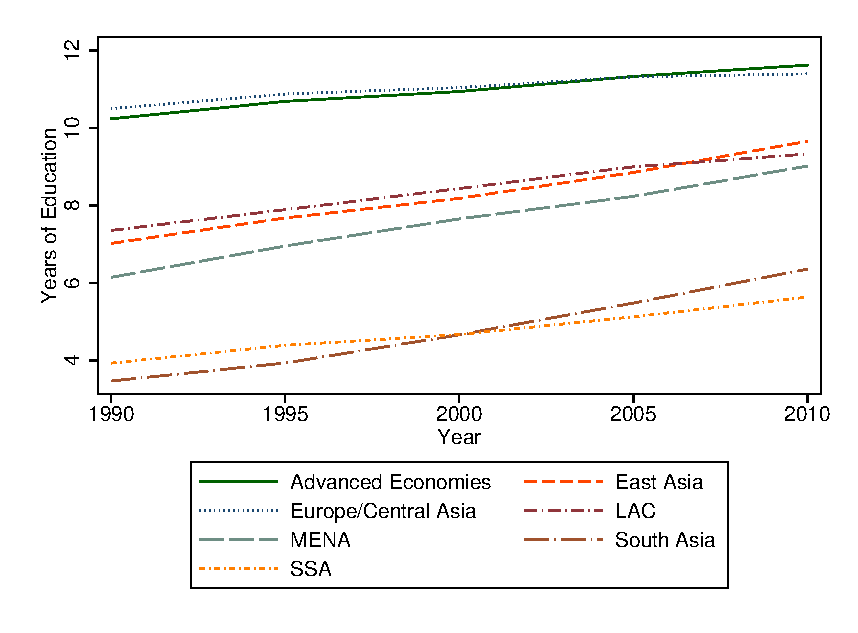
\includegraphics[scale=0.9]{\MMRfolder/Results/graphs/trends/SchoolingRegion.eps} 
\end{center}
\end{figure}

\begin{figure}[h!]
\begin{center}
\caption{Maternal Mortality Ratio by Region: 1990-2010}
\label{fig:MMRRegion}
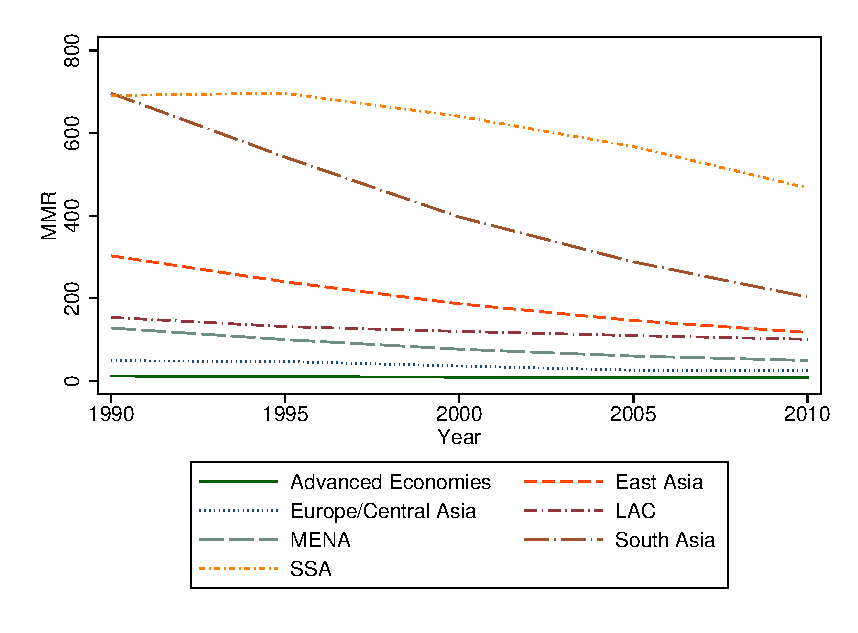
\includegraphics[scale=0.9]{\MMRfolder/Results/graphs/trends/MMRRegion.eps} 
\end{center}
\end{figure}

\begin{figure}[h!]
\begin{center}
\caption{Maternal Mortality and Education: Functional Form}
\label{fig:educmmr}
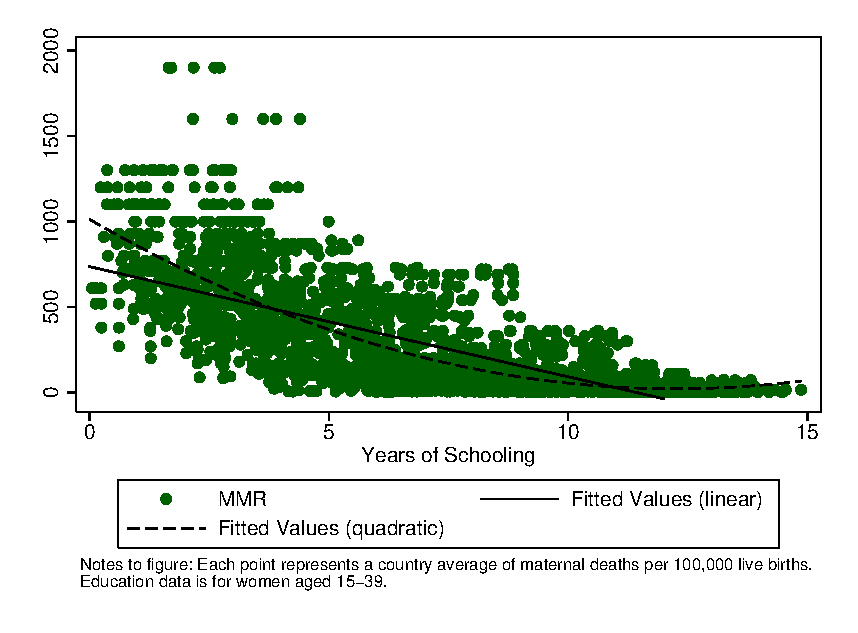
\includegraphics[scale=0.9]{\MMRfolder/Results/graphs/trends/Schooling_MMR_F.eps} 
\end{center}
\end{figure}

\begin{landscape}
\begin{figure}[h!]
\begin{center}
\caption{Maternal Mortality Ratio by Country}
\label{fig:MMRGlobal}
\includegraphics[scale=0.9]{\MMRfolder/Results_aug2013/Graphs/MMR_2010.eps} 
\end{center}
\end{figure}
\end{landscape}



\newpage
\bibliography{./Paper/BibTeX}


\end{spacing}
\end{document}
